%\chapter{Wykonanie testów i dokonanie odpowiednich pomiarów}
%\section{Opis metodyki testowania}
%\section{Przebieg testów}
%\section{Analiza wyników}

\chapter{Pomiary testowe}

W celu weryfikacji poprawności działania pirometru, przeprowadzono test porównawczy z wykorzystaniem wzorcowanego pirometru przemysłowego Sonel DIT-200 wraz z opcją pomiaru temperatury metodą stykową co pokazano na zdjęciu \ref{fig:pomiar}. Test przeprowadzono w kontrolowanych warunkach laboratoryjnych w przedziale temperatury 25 - 30°C. Zakres temperatury mierzonego obiektu wynosi od 35°C do 160°C. Obiektem pomiarowym jest płyta grzejna o mocy 800W, pomalowanego na kolor czarny matowy.

\vspace{12pt}

Procedura testowa:
\begin{enumerate}
\item Przygotowanie stanowiska składającego się z urządzenia testowanego,  pirometru przemysłowego wyposażonego w pomiar metodą optyczną oraz stykową oraz obiektu odwzorowującego wymagane nastawy temperatury. \item Wykonanie pomiarów temperatury w zakresie od 35°C do 160°C w odstępach co 5°C oraz zarejestrowanie ich w arkuszu kalkulacyjnym. %\item Dwukrotne powtórzenie pomiarów. Każdy pomiar był wykonywany trzykrotnie, a wyniki uśredniano w celu zwiększenia dokładności pomiarów.
\end{enumerate}

\newpage

%\section{Tabela porównawcza pomiarów}

\begin{table}[h!]
    \centering
    \begin{tabularx}{\textwidth}{|C|C|C|} % Użycie nowego typu kolumny
    \hline
    \textbf{Temperatura z Arduino [°C]} & 
    \textbf{Termometr stykowy [°C]} & 
    \textbf{Pirometr przemysłowy [°C]} \\
    \hline
    160 & 160 & 164.7 \\
    \hline
    155 & 156.1 & 159.3 \\
    \hline
    150 & 151.8 & 156.6 \\
    \hline
    145 & 146.9 & 152.9 \\
    \hline
    140 & 142.5 & 147.2 \\
    \hline
    135 & 137.2 & 142.1 \\
    \hline
    130 & 132.5 & 139.2 \\
    \hline
    125 & 127.8 & 131.3 \\
    \hline
    120 & 122.3 & 126.3 \\
    \hline
    115 & 117.4 & 120.5 \\
    \hline
    110 & 112.7 & 115.6 \\
    \hline
    105 & 106.9 & 110.7 \\
    \hline
    100 & 101 & 105 \\
    \hline
    95 & 94.8 & 100 \\
    \hline
    90 & 89.7 & 96.2 \\
    \hline
    85 & 83.8 & 92.4 \\
    \hline
    80 & 79.3 & 88.5 \\
    \hline
    75 & 73.3 & 84.1 \\
    \hline
    70 & 68.7 & 80.1 \\
    \hline
    65 & 63.8 & 75.7 \\
    \hline
    60 & 58.7 & 70.7 \\
    \hline
    55 & 54.1 & 66 \\
    \hline
    50 & 51 & 60.4 \\
    \hline
    45 & 45.4 & 54.2 \\
    \hline
    40 & 41.1 & 42.1 \\
    \hline
    35 & 37 & 36.1 \\
    \hline
    \end{tabularx}
    \caption{Porównanie wyników pomiarów z pirometru Arduino, pirometru przemysłowego oraz termometru stykowego}
    \label{tab:porownanie_pomiarow}
    \end{table}

    \begin{figure}[h!]
        \centering
        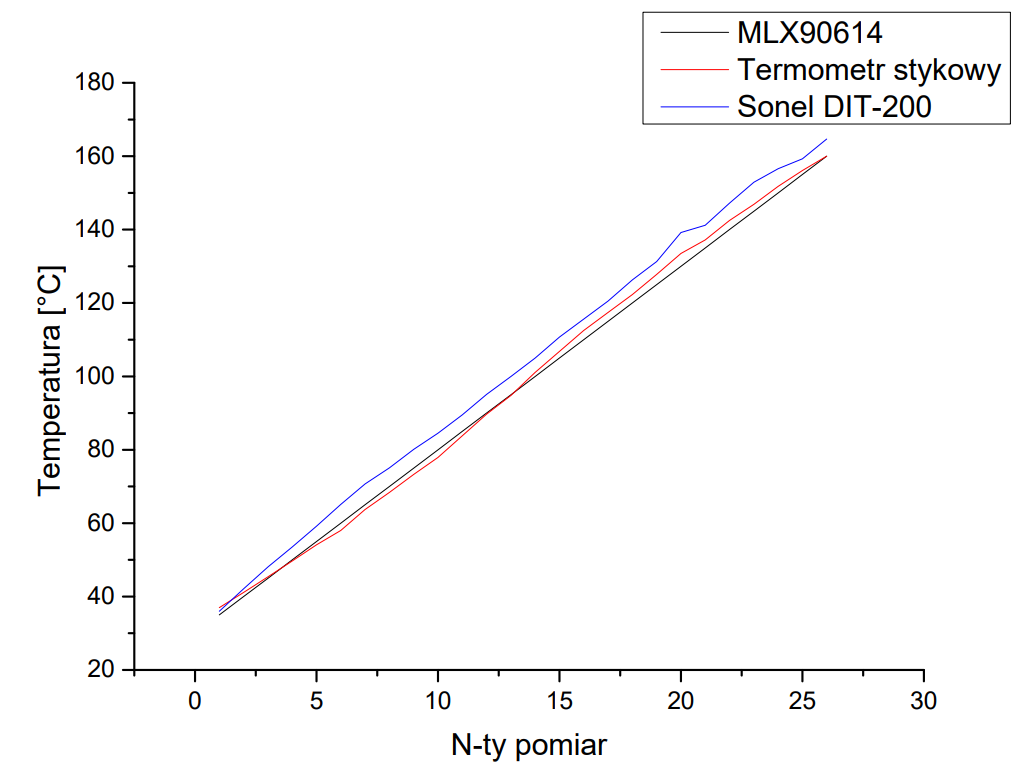
\includegraphics[width=1.05\textwidth]{images/wykres.png}
        \caption{Wizualizacja wyników pomiarów}
        \label{fig:origin}
    \end{figure}

\begin{figure}[h!]
    \centering
    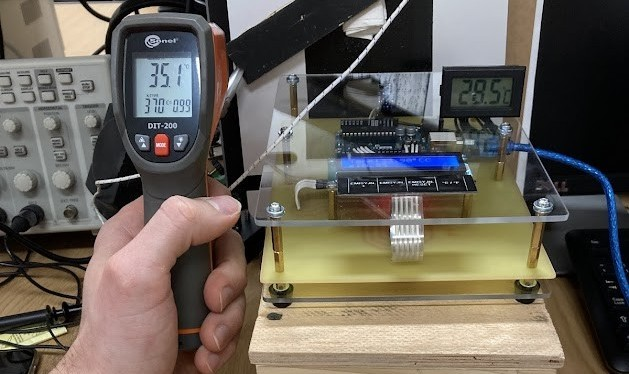
\includegraphics[width=1.05\textwidth]{images/test.jpg}
    \caption{Przebieg procedury testowej}
    \label{fig:pomiar}
\end{figure}

Wykorzystane przyrządy pomiarowe oraz ich najważniejsze parametry zostały przedstawione w tabeli \ref{tab:parametry_termometrow}.

\vspace{12pt}

Rysunek \ref{fig:origin} przedstawia wizualizację wyników pomiarów. Na podstawie przeprowadzonych testów można stwierdzić, że pirometr spełnia założenia projektowe i może być stosowany do bezkontaktowego pomiaru temperatury w zakresie od 35°C do 160°C.

\begin{table}[h!]
    \centering
    \begin{tabularx}{\textwidth}{|C|C|C|C|} % Użycie nowego typu kolumny
    \hline
    \textbf{Parametr} & \textbf{Termometr stykowy} & \textbf{Sonel DIT-200} & \textbf{MLX90614} \\
    \hline
    Zakres temperatur & -50°C do 150°C & -50°C do 1000°C & -70°C do 380°C \\
    \hline
    Dokładność & ±0.5°C & ±1.5°C & ±0.5°C \\
    \hline
    Rozdzielczość & 0.1°C & 0.1°C & 0.1°C \\
    \hline
    Czas odpowiedzi & 1 s & 500 ms & 100 ms \\
    \hline
    Emisyjność & N/A & 0.1 do 1.0 regulowana & 0.00 do 1.00 regulowana programowo \\
    \hline
    Typ czujnika & Termistor & Pirometr & Pirometr \\
    \hline
    Interfejs & Analogowy & Cyfrowy & I2C \\
    \hline
    \end{tabularx}
    \caption{Porównanie parametrów termometra stykowego, termometra przemysłowego Sonel DIT-200 i MLX90614 \cite{9} \cite{10}}
    \label{tab:parametry_termometrow}
    \end{table}

\newpage

    \section*{Opis przebiegu na wykresie}

    Wykres \ref{fig:origin} przedstawia porównanie temperatur mierzonych za pomocą trzech różnych urządzeń pomiarowych w funkcji liczby kolejnych pomiarów (\textit{N-ty pomiar}):
    
    \begin{itemize}
        \item \textbf{MLX90614} (czarna linia): Czujnik bezkontaktowy do pomiaru temperatury.
        \item \textbf{Termometr stykowy} (czerwona linia): Tradycyjny termometr stykowy mierzący temperaturę po kontakcie z obiektem.
        \item \textbf{Sonel DIT-200} (niebieska linia): Precyzyjne narzędzie pomiarowe.
    \end{itemize}
    
    \subsection*{Obserwacje}
    
    \begin{itemize}
        \item Wszystkie trzy urządzenia pokazują bardzo zbliżone wartości temperatury w całym zakresie pomiarowym.
        %\item Dane wskazują na liniowy wzrost temperatury w miarę wzrostu liczby pomiarów.
        \item Różnice między liniami są minimalne, jednak można zauważyć, że:
        \begin{itemize}
            \item \textbf{Sonel DIT-200} (niebieska linia) wykazuje nieco wyższe wartości niż pozostałe urządzenia w środkowej części zakresu (np. pomiary od 10 do 20).
            \item \textbf{Termometr stykowy} (czerwona linia) znajduje się między czujnikiem \textbf{MLX90614} a urządzeniem \textbf{Sonel DIT-200}.
            \item \textbf{MLX90614} (czarna linia) ma najniższe wskazania w porównaniu do pozostałych urządzeń.
        \end{itemize}
    \end{itemize}
    
    \subsection*{Wnioski}
    
    Wyniki mogą sugerować niewielkie różnice w dokładności lub metodologii pomiarowej pomiędzy urządzeniami. Wszystkie jednak zapewniają spójne dane, co wskazuje, że każde z urządzeń można używać do pomiaru temperatury w danym zakresie z wysoką pewnością.
    

\chapter*{Wyprowadzenie wzoru na emisyjność badanego obiektu}
Poniżej przedstawiono zestaw wzorów opisujących promieniowanie cieplne oraz związane z nimi parametry fizyczne:
\begin{itemize}
    %\item \(\sigma\) – stała Stefana-Boltzmanna, określająca intensywność promieniowania ciała doskonale czarnego,
    \item \(\epsilon\) – współczynnik emisyjności (od 0 do 1), opisujący zdolność ciała do emitowania promieniowania w stosunku do ciała doskonale czarnego,
    %\item \(S\) – powierzchnia ciała emitującego promieniowanie,
    \item \(T_{\text{env}}\) – temperatura otoczenia w stopniach Celcjusza (°C),
    \item \(T_{\text{meas}}\) – zmierzona temperatura obiektu stopniach Celcjusza (°C),
    \item \(T_{\text{real}}\) – rzeczywista temperatura obiektu stopniach Celcjusza (°C).
\end{itemize}
%\newpage
%\section{Wzory}
%1. Moc promieniowania cieplnego emitowanego przez ciało:
%\[
%P = \sigma \cdot \epsilon \cdot S \cdot \left( T_{\text{env}}^4 - T^4 \right)
%\]
%1. 
%Równanie równowagi cieplnej opisujące emisję promieniowania:
%\[
%\epsilon \cdot T_{\text{env}}^4 - \epsilon \cdot T_{\text{real}}^4 = T_{\text{env}}^4 - T_{\text{meas}}^4
%\]
%2. 
Współczynnik emisyjności obliczony na podstawie temperatur:
\[
\epsilon = \frac{T_{\text{env}}^4 - T_{\text{meas}}^4}{T_{\text{env}}^4 - T_{\text{real}}^4}
\]
Na podstawie dwóch różnych temperatur wyznaczono emisyjność badanego obiektu. 

Wzory zostały zastosowane do obliczenia wartości emisyjności:
\[
\epsilon = \frac{30.15^4 - 69.31^4}{30.15^4 - 70.1^4} = 0.9541
\]
Po zaokrągleniu do czterech miejsc po przecinku wynik to: 0.9541.